\documentclass[12pt,a4paper]{article}
%\usepackage{ctex}
\usepackage{amsmath,amscd,amsbsy,amssymb,latexsym,url,bm,amsthm}
\usepackage{epsfig,graphicx,subfigure}
\usepackage{enumitem,balance}
\usepackage{wrapfig}
\usepackage{mathrsfs,euscript}
\usepackage[x11names,svgnames,dvipsnames]{xcolor}
\usepackage{hyperref}
\usepackage[vlined,ruled,commentsnumbered,linesnumbered]{algorithm2e}
\usepackage{listings}
\usepackage{multicol}
%\usepackage{fontspec}

\renewcommand{\listalgorithmcfname}{List of Algorithms}
\renewcommand{\algorithmcfname}{Alg.}
\newtheorem{theorem}{Theorem}
\newtheorem{lemma}[theorem]{Lemma}
\newtheorem{proposition}[theorem]{Proposition}
\newtheorem{corollary}[theorem]{Corollary}
\newtheorem{exercise}{Exercise}
\newtheorem*{solution}{Solution}
\newtheorem{definition}{Definition}
\theoremstyle{definition}


%\numberwithin{equation}{section}
%\numberwithin{figure}{section}

\renewcommand{\thefootnote}{\fnsymbol{footnote}}

\newcommand{\postscript}[2]
 {\setlength{\epsfxsize}{#2\hsize}
  \centerline{\epsfbox{#1}}}

\renewcommand{\baselinestretch}{1.0}

\setlength{\oddsidemargin}{-0.365in}
\setlength{\evensidemargin}{-0.365in}
\setlength{\topmargin}{-0.3in}
\setlength{\headheight}{0in}
\setlength{\headsep}{0in}
\setlength{\textheight}{10.1in}
\setlength{\textwidth}{7in}
\makeatletter \renewenvironment{proof}[1][Proof] {\par\pushQED{\qed}\normalfont\topsep6\p@\@plus6\p@\relax\trivlist\item[\hskip\labelsep\bfseries#1\@addpunct{.}]\ignorespaces}{\popQED\endtrivlist\@endpefalse} \makeatother
\makeatletter
\renewenvironment{solution}[1][Solution] {\par\pushQED{\qed}\normalfont\topsep6\p@\@plus6\p@\relax\trivlist\item[\hskip\labelsep\bfseries#1\@addpunct{.}]\ignorespaces}{\popQED\endtrivlist\@endpefalse} \makeatother


\definecolor{codegreen}{rgb}{0.44,0.68,0.28}
\definecolor{codegray}{rgb}{0.5,0.5,0.5}
\definecolor{codepurple}{rgb}{0.58,0,0.82}
\definecolor{backcolour}{rgb}{0.96,0.96,0.96}

\lstset{
language=C++,
frame=shadowbox,
keywordstyle = \color{blue}\bfseries,
commentstyle=\color{codegreen},
tabsize = 4,
backgroundcolor=\color{backcolour},
numbers=left,
numbersep=5pt,
breaklines=true,
emph = {int,float,double,char},emphstyle=\color{orange},
emph ={[2]const, typedef},emphstyle = {[2]\color{red}} }



\begin{document}
\noindent

%========================================================================
\noindent\framebox[\linewidth]{\shortstack[c]{
\Large{\textbf{Lab08-Graphs}}\vspace{1mm}\\
VE281 - Data Structures and Algorithms, Xiaofeng Gao, TA: Li Ma, Autumn 2019}}
%CS26019 - Algorithm Design and Analysis, Xiaofeng Gao, Autumn 2019}}
\begin{center}
\footnotesize{\color{red}$*$ Please upload your assignment to website. Contact webmaster for any questions.}

\footnotesize{\color{blue}$*$ Name:Wu Jiayao \quad Student ID:517370910257 \quad Email: jiayaowu1999@sjtu.edu.cn}
\end{center}


\begin{enumerate}

\item \textbf{DAG.} Suppose that you are given a directed acyclic graph $G=(V,E)$ with real-valued edge weights and two distinct nodes $s$ and $d$. Describe an algorithm for finding a longest weighted simple path from $s$ to $d$. For example, for the graph shown in Figure 1, the longest path from node $A$ to node $C$ should be $A \rightarrow B \rightarrow F \rightarrow C$. If there is no path exists between the two nodes, your algorithm just tells so. What is the efficiency of your algorithm? (Hint: consider topological sorting on the DAG.)

\begin{solution}
\begin{flushleft}
\end{flushleft}
Denote $<u,v>$ the edge goes from u to v.  \\
\begin{algorithm}[H]
  \KwIn{A DAG $G$, points $s$, $d$}
  \KwOut{The longest path from $s$ to $d$}
  Made a copy of $G$ to do topological sort. \\
  $visitNum$ $\gets$ $0$ \\
  $H$ $\gets$ $\{\}$ \\
  \While{$E$ $\neq$ $\emptyset$}{
      $v$ $\gets$ a vertex in V that no edge points to it \\
      $visitNum++$ \\
      $H[visitNum]$ $\gets$ $v$ \\
      $V$ $\gets$ $V  \backslash v$ \\
      \For {vertex $u$ in $V$}{
          \If{edge $<v,u>$ exists}{
              $E$ $\gets$ $E \backslash <v,u>$
          }
      }
  }
  \ForEach{$v$ in $G.V$}{
    $v.pathLength=\infty$
  }
  \ForEach( // Visit in topological order){$u$ in H}{
    \ForEach{$edge<u,v>$}{
      \If{$v.pathLength < u.pathLength + edge<v,i>.weight$}{
        $u.pathLength=v.pathLength + edge<v,i>.weight$ \\
        $v.prev=u$ \\
      }
    }
  }
  \If{$d.pathLength=\infty$}{
    \Return{Not found}
  }
  $itr = d$ \\
  $path=[]$ \\
  \While{$True$}{
    push $itr$ into the front of $path$ \\
    \If{$itr==s$}{
      break
    }
    $itr=itr.prev$
  }
  \Return{path}
\end{algorithm}
The time complexity is $\mathcal{O}(|V|+|E|)$, where $\mathcal{O}(|V|)$ for topological sort, $\mathcal{O}(|E|)$ for path length determination. \\
\end{solution}
\begin{figure}[htbp]
% \begin{minipage}[t]{0.5\linewidth}
% \centering
% 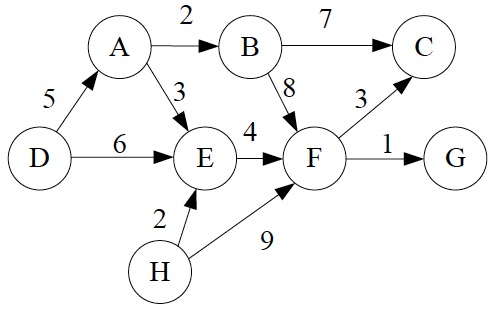
\includegraphics[scale=0.35]{Lab08-figure1.jpg}
% \caption{A weighted undirected graph.}
% \end{minipage}%
% \begin{minipage}[t]{0.5\linewidth}
\centering
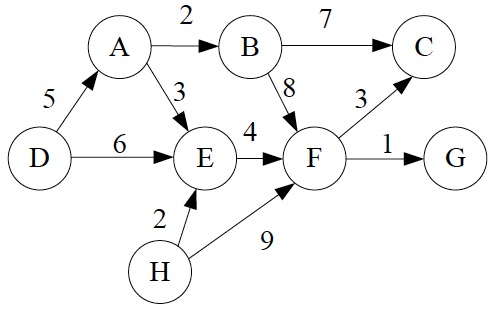
\includegraphics[scale=0.35]{Lab08-figure1.jpg}
\caption{A weighted directed graph.}
% \end{minipage}
\end{figure}

\item \textbf{ShortestPath.} Suppose that you are given a directed graph $G=(V,E)$ on which each edge $(u,v) \in E$ has an associated value $r(u,v)$, which is a real number in the range $0 \leq r(u,v) \leq 1$ that represents the reliability of a communication channel from vertex $u$ to vertex $v$. We interpret $r(u,v)$ as the probability that the channel from $u$ to $v$ will not fail, and we assume that these probabilities are independent. Give an efficient algorithm to find the most reliable path between two given vertices.

\begin{solution}
  \begin{flushleft}
  \end{flushleft}
  \begin{algorithm}[H]
    \KwIn{A Graph $G$, points $s$, $d$}
    \KwOut{The most reliable path from $s$ to $d$}
    Set a priotity queue $pq$, where the value is the edges, the key is the current probability of $v$, $v.p$, in the edge, edge with the largest probability $v$ is on the top. \\
    visit[s] = 1 \\
    $s.pathLength = 1$ \\
    \ForEach(foreach-comment){$edge<s,i>$}{
      $i.p = s.p \times r(s,i)$ \\
      $i.prev = s$ \\
      push $(s,i)$ into $pq$  \\
  
    }
    \While{$pq$ is not empty}{
      $(u,v)$ = pq.dequeue \\
      \If{$visit[v]==1$}{
        continue
      }
      \ForEach{$(v,i)$}{
        \If{$visit[i]==0$ and $i.p < v.p \times r(v,i)$}{
          $i.p=v.p \times r(v,i)$ \\
          $visit[i] = 1$ \\
          $i.prev=v$ \\
          push $(v,i)$ into $pq$ \\
        }
      }
    }
    $itr = d$ \\
    $path=[]$ \\
    \While{$True$}{
      push $itr$ into the front of $path$ \\
      \If{$itr==s$}{
        break
      }
      $itr=itr.prev$
    }
    \Return{path}
  \end{algorithm}
  \end{solution}

\item \textbf{GraphSearch.} Let $G=(V,E)$ be a connected, undirected graph. Give an $O(|V|+|E|)$-time algorithm to compute a path in $G$ that traverses each edge in $E$ \textbf{exactly once in each direction}. For example, for the graph shown in Figure 2, one path satisfying the requirement is
$$A \rightarrow B \rightarrow C \rightarrow D \rightarrow C \rightarrow A \rightarrow C \rightarrow B \rightarrow A$$
Note that in the above path, each edge is visited exactly once in each direction.

\begin{figure}[h]
 \centering
 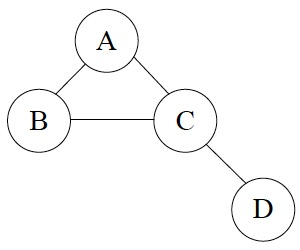
\includegraphics[scale=0.35]{Lab08-figure2.jpg}
 \caption{A undirected graph.}
\end{figure}

\begin{solution}
\begin{flushleft}
  
\end{flushleft}
\begin{algorithm}[H]
\KwIn{An undirected graph $G<V,E>$}
\KwOut{A path}
Reconstruct the graph into a directed graph, as one undirected edge(u,v) means to directed edges (u,v),(v,u)\\
path=[] \\
Create a stack $q$ \\
$visit[v] = 0$ for all vertices \\
$prev[v] = v$ for all vertices \\
Push a vertice $U$ that has an edge in $G.E$ \\
\While{$q$ is not empty}{
    $u=q.dequeue$ \\
    Append $u$ to $path$ \\
    $visit[u] = 1$ \\
    \ForEach{$edge<u,v>$}{
        \If{$visit[v]== 0$}{
            push $v$ into $q$ \\
            $prev[v] = u$ \\
            $G.E \gets G.E \backslash <u,v>$
        }
        \Else{
            \If{$prev[u] != v$}{
              Append $[v,u]$ into the path \\
              $G.E \gets G.E \backslash <u,v>$ \\
              $G.E \gets G.E \backslash <v,u>$ \\
            }
            
        }
        
    }
}
\Return{path}
\end{algorithm}
\end{solution}

\end{enumerate}

%========================================================================
\end{document}
